\titlespacing\section{\parindent}{0pt}{12pt}
\section{Классификация существующих решений}
\titlespacing\subsection{\parindent}{0pt}{24pt}
\subsection{Парольная аутентификация}
Парольная аутентификация \cite{bib2} --- аутентификация на основе обладания неким секретным знанием. 
В большинстве случаев пароли могут обеспечить достаточный уровень защиты системы, но в крупных организациях применение многоразовых паролей не обеспечивает необходимой безопасности.

Аутентификация на основе открытого пароля является самым старым и простым методом.

Принцип работы:

\begin{enumerate}
    \item пользователь вводит свое имя и пароль на рабочей станции;
    \item имя и пароль передаются в открытом доступе по сети;
    \item сервер аутентификации находит учетную запись пользователя в базе данных аутентификации и сравнивает введенные данные с ее содержимым. 
\end{enumerate}

Усовершенствованным вариантом многоразового пароля является использование его хэш-значения, получаемого с помощью криптографической хэш-функции.

Принцип работы:
\begin{enumerate}
    \item пользователь вводит свое имя и пароль на рабочей станции;
    \item рабочая станция вычисляет от введенного пароля хэш-значение;
    \item имя и хэш-значение передаются в открытом доступе по сети серверу аутентификации;
    \item cервер аутентификации сравнивает результат хэш-значения от введенного пользователем пароля с хэш-значением, хранящимся в учетной записи пользователя. 
\end{enumerate}

Так как невозможно восстановить исходный пароль даже при владении \linebreak хэш-значением, то вероятность доступа к информации ограниченного доступа злоумышленником минимальна.

PIN-код \cite{bib2} --- это разновидность пароля, который в основном используют для аутентификации на локальном устройстве.

Отличие PIN-кода от пароля в условиях и области его использования. PIN-код можно ввести только с использванием клавиатуры конкретного устройства, то есть его не передают по сети, поэтому никто не может его перехватить.

\titlespacing\subsection{\parindent}{24pt}{24pt}
\subsection{Аутентификация с помощью биометрических характеристик}
Биометрическая характеристика \cite{bib2} --- это измеримая физиологическая или поведенческая черта живого человека, которую можно использовать для установления личности или проверки декларируемых личных данных.

Биометрические характеристики делятся на два вида: физиологические и поведенческие.

Физиологическими характеристиками являются данные, полученные измерением анатомических характеристик человека.

К физиологическим характеристикам относятся:
\begin{itemize}
    \item [---] отпечаток пальца;
    \item [---] радужная оболочка глаза;
    \item [---] сетчатка глаза;
    \item [---] геометрия рук;
    \item [---] лицо.
\end{itemize}

Поведенческими характеристиками являются данные, полученные измерением действий человека.

К поведенческим характеристикам относятся:

\begin{itemize}
    \item [---] голос;
    \item [---] подпись;
    \item [---] ритм работы сердца;
    \item [---] динамика работы на клавиатуре.
\end{itemize}

Все биометрические системы имеют одинаковый принцип работы. Пользователь предоставляет образец биометрической характеристики, регистрирующее устройство обрабатывает его, в результате получается контрольный шаблон. Под шаблоном подразумевается большая числовая последовательность. 

При регистрации в биометрической системе на основе нескольких образцов создается эталонный шаблон, с которым и производится сравнение контрольного шаблона. Поскольку они никогда не смогут совпасть, необходимо настроить пороговую величину, которую степень совпадения должна превысить.

На рисунке \ref{fig:biometric} изображена базовая схема работы биометрической системы.

\begin{figure}[h]
    \centering
    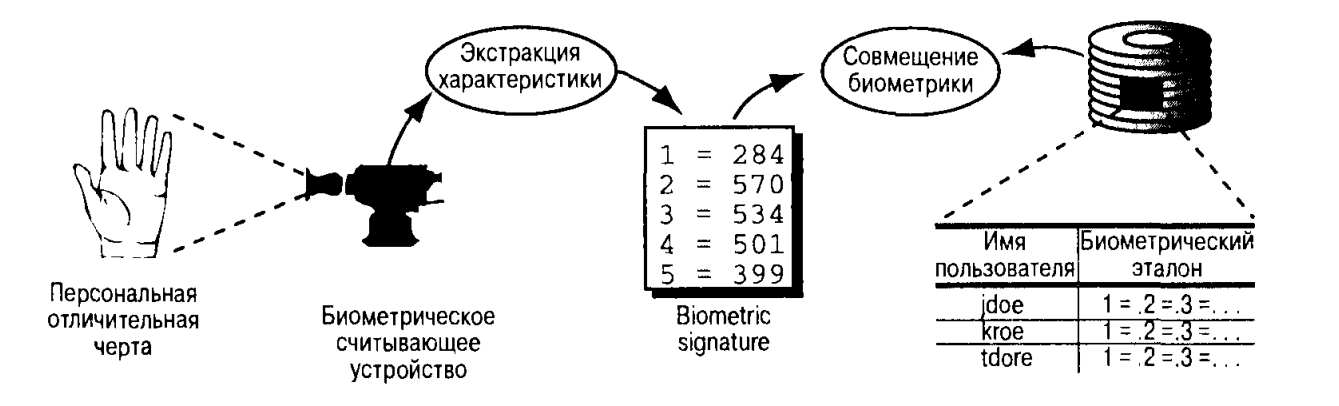
\includegraphics[width=\textwidth]{img/biometric.png}
    \caption{Схема работы биометрической системы \cite{bib2}}
    \label{fig:biometric}
\end{figure}

Главными, для оценки точности биометрических систем, являются два параметра \cite{bib7}:

FAR --- коэффициент ложного пропуска, т.е. процент возникновения ситуаций, когда система разрешает доступ пользователю, который незарегистрирован в системе.

FRR --- коэффициент ложного отказа, т.е. отказ в доступе пользователю, который зарегистрирован в системе.

Так как все люди обладают индивидуальными характеристиками, а украсть или подменить их практически невозможно, то данный метод можно считать устойчивым к злоумышленным действиям. Однако существуют другие проблемы, например: некоторые люди не имеют частей тела, необходимых для внесения в систему, есть и те, кто считают, что сбор биометрических данных --- это вмешательство в их частную жизнь или это оскорбляет их культурные или религиозные ценности.

\titlespacing\subsection{\parindent}{24pt}{24pt}
\subsection{Аутентификация с помощью одноразовых паролей}
Одноразовые пароли \cite{bib2} --- динамическая аутентификационная информация, генерируемая для единственного использования с помощью аутентификационных устройств (программных или аппаратных).

Такие устройства называются OTP-токенами. Для генерации одноразовых паролей OTP-токены используют хэш-функции или криптографические алгоритмы. Обычно в OTP-токенах применяют симметричную криптографию \linebreak (криптографию с одним ключом). Устройство пользователя содержит уникальный секретный ключ, используемый для шифрования некоторых данных для генерации OTP. Такой же ключ хранится на сервере аутентификации, там он шифруется. В итоге, сравниваются два результата шифрования: если совпали, значит аутентификация прошла успешно.

Методы, используюмые OTP-токенами, которые применяют симметричную криптографию, можно разделить на две группы, работающие: в асинхронном и в синхронном режимах. 

В асинхронном режиме работает метод <<запрос-ответ>>, а методы <<только ответ>>, <<синхронизация по времени>> и <<синхронизация по событию>> в синхронном режиме.

В методе <<запрос-ответ>> OTP является ответом пользователя на случайный запрос от сервера аутентификации.

В методе <<только ответ>> аутентификационное устройство и сервер аутентификации генерирует <<скрытый>> запрос, используя значения предыдущего запроса. Чтобы изначально инициализировать данный процесс используют уникальное случайное начальное значение, которое генерируется при инициализации OTP-токена. 

В методе <<синхронизация по времени>> OTP генерируется на основе значения внутренних часов аутентификационного устройства и аутентификационного сервера. 

В методе <<синхронизация по событию>> OTP-токен и сервер аутентификации ведут количественный учет прохождения аутентификации данным пользователем, и на основе этого числа генерируют OTP.

\titlespacing\subsection{\parindent}{24pt}{24pt}
\subsection{Аутентификация с помощью открытого ключа}
В криптографии с открытым ключом (асимметричная криптография) алгоритмы используют связанные между собой пары ключей, состоящие из открытого и закрытого ключа \cite{bib2}. Информация, зашифрованная с помощью одного ключа из ключевой пары, может быть расшифрована только с помощью другого ключа из это же пары.

Идея в том, что аутентификационный сервер хранит файл всех открытых ключей, а пользователь сам хранит свой закрытый ключ.

Принцип работы:
\begin{enumerate}
    \item сервер посылает пользователю случайную строку, созданную генератором случайных чисел;
    \item пользователь шифрует эту строку своим закрытым ключом и посылает ее обратно серверу вместе со своим именем;
    \item сервер находит в базе данных открытый ключ пользователя и расшифровывает сообщение, используя этот открытый ключ;
    \item если отправленная и расшифрованная строки совпадают, сервер предоставляет пользователю доступ к системе. 
\end{enumerate}

Такой вид аутентификации может быть надежным, однако необходимо решить проблему с безопасным хранением закрытого ключа. Самый простой вариант --- это хранить закрытый ключ внутри локального хранилища операционной системы, которое защищено с помощью криптографических методов. Однако жесткий диск уязвим к прямым и сетевым атакам, и в данном случае ключ связан с конкретным компьютером. Решение --- специализированные устройства. 

Далее были рассмотрены основные виды таких устройств.

Таблетка Touch Memory \cite{bib2} --- это электронное устройство, имеющее энергонезависимую память, размещенную в металлическом корпусе, в которой можно хранить данные пользователя. Устройство активизируется в момент контакта со считывателем.

Смарт-карта \cite{bib2} --- это пластиковая карта, со встроенной микросхемой, микропроцессором и операционной системой, контролирующей устройство и доступ к объектам в памяти. Зачастую она могжет проводить криптографические вычисления.

Все смарт-карты можно разделить на три вида \cite{bib8}:
\begin{enumerate}
    \item контактные карты памяти --- могут работать, когда электрические контакты, расположенные на поверхности, соприкасаются со считывателем;
    \item бесконтактная смарт-карта ---  информация считывается с карты, если \linebreak устройство использует определённую радиочастоту (RFID), поэтому физический контакт со считывателем не нужен;
    \item многокомпонентная карта --- это редко встречающийся тип карт, который создаётся под какое-то конкретное решение, например, может быть встроен считыватель отпечатка пальца.
\end{enumerate}

USB-ключ \cite{bib2} --- аппаратное устройство, со встроенной микросхемой, которое хранит в себе ключ, доступ к которому осуществляется через порт USB. 

Смарт-карты и USB-ключи являются интеллектуальными устройствами.

Чтобы использовать закрытый ключ, с устройства можно либо его экспортировать, и криптографические операции осуществлять уже на рабочей станции, либо все вычисления проделать на самом устройстве. Второй вариант является наиболее безопасным.

Слабым местом любых токенов, при всем совершенстве применяемых алгоритмов является возможность утери или целенаправленного хищения, либо уничтожения ключевого носителя.

\titlespacing\subsection{\parindent}{24pt}{24pt}
\subsection{Аутентификация через географическое местоположение}
Данный метод использует GPS. GPS состоит из 24 спутников, положение которых на орбите всегда точно известно. Каждый спутник передает непрерывный поток идентифицирующей информации, которая при объединении с сигналами от других видимых спутников позволяет точно определить географическое местонахождение \cite{bib3}. 
Основным достоинством такого метода является то, что аппаратура GPS надежна в использовании и относительно недорога. Ее использование необходимо в тех случаях, когда пользователь должен находиться в нужном месте, например офисном здании. Так как координаты спутников меняются постоянно, то вероятность перехвата этих координат равна нулю. 

\titlespacing\subsection{\parindent}{24pt}{24pt}
\subsection{Графическая аутентификация}
Графическая аутентификация \cite{bib3} --- это метод аутентификации, когда для доступа в систему пользователю необходимо выполнить некоторые операции над изображениями. 

Далее были рассмотрены некоторые схемы аутентификации на основе графических паролей.

В схеме \textit{Passlogix} \cite{bib9} при генерации пароля пользователю показывают картинку, он выбираете на ней несколько мест и нажимет на них мышью. Парольная комбинация строится из 5-6 кликов мышки в определенном порядке. При вводе пароля показывается та же самая картинка, и надо нажать в те же самые места. Допускается, что при аутентификации пользователь попадает хотя бы в окрестность парольных точек. Точки и последовательность их нажатия хранятся в хэшированном виде. 

У \textit{Passlogix} есть свои плюсы и минусы. Если в качестве картинки выбрать большую фотографию со множеством мелких деталей - например, городской пейзаж в высоком разрешении, то даже четыре клика на нем окажутся паролем, легким для запоминания, но очень трудным для грубого взлома. Если же, наоборот, выбрать небольшой портрет человека, с двумя родинками и кольцом на руке, то не составит труда перебрать наиболее вероятные варианты пароля.

Схема \textit{PassFaces} \cite{bib9} основана на распознавании человеческих лиц. Во время создания пароля пользователям предоставляется большой набор изображений на выбор. Чтобы войти в систему, пользователь должен узнать предварительно выбранное лицо из нескольких представленных ему. Лица появляются в случайных позициях.

В схеме \textit{Pass-string} \cite{bib9} \textit{N} объектов случайно разбросано на экране. Пользователь выбирает \textit{K} объектов (пропускное подмножество) и запоминает их. Существуют разные варианты для входа: найти 3 парольных объекта, используя прямые мысленно их соединить и нажать внутри фигуры или щелкнуть объект на пересечении прямых, которые проходят через четыре парольных объекта.

В схеме \textit{Deja Vu} \cite{bib9} пользователь запоминает \textit{M} изображений (пропускное подмножество) из \textit{P} возможных. Чтобы войти пользователь должен правильно выбрать изображения, которые состоят в его пропускном подмножестве.

\titlespacing\subsubsection{\parindent}{24pt}{24pt}
\subsection{Сравнение методов аутентификации}
Сокращения для категорий:
\begin{itemize}
    \item [---] ПА --- парольная аутентификация;
    \item [---] БА --- биометрическая аутентификация;
    \item [---] ОП --- аутентификация с помощью одноразовых паролей;
    \item [---] ОК --- аутентификация с помощью открытого ключа;
    \item [---] ГМ --- аутентификация через географическое местоположение;
    \item [---] ГА --- графическая аутентификация.
\end{itemize}

Сокращения для критериев:
\begin{itemize}
    \item[---] К1 --- стоимость установки и обслуживания (затраты времени, усилий и денежных средств);
    \item[---] К2 --- удобство использования (простота и портативность системы);
    \item[---] К3 --- возможность возникновения ошибок (подразумевается возможность допустить к системе незарегистрированного пользователя или не допустить зарегистрированного пользователя);
    \item[---] К4 --- требование наличия дополнительных программных и аппаратных средств;
    \item[---] А1 --- возможность полного перебора;
    \item[---] А2 --- возможность подглядеть из-за плеча;
    \item[---] А3 --- возможность перехвата пароля;
    \item[---] A4 --- возможность троянского коня.
\end{itemize}

Классификацию рассмотренных методов аутентификации можно увидеть в таблицах \ref{tabular:res1} и \ref{tabular:res2}.

\begin{table}[h]
    \begin{center}
    \begin{threeparttable}
    \captionsetup{justification=raggedright,singlelinecheck=off}
        \caption{\label{tabular:res1} Классификация методов аутентификации пользователя по качественным характеристикам.}
        \begin{tabular}{|c|c|c|c|c|}
            \hline
            \bfseries Метод аутентификации & \bfseries К1 & \bfseries К2 & \bfseries К3 & \bfseries К4  \\
            \hline
            ПА & Низкая & Среднее & Нет & Не требуется \\ \hline
            БА & Высокая & Высокое & Да & Требуется АО \\ \hline
            ОП & Низкая & Низкое & Нет & Требуется \\ \hline
            ОК & Средняя & Среднее & Нет & Требуется \\ \hline
            ГМ & Средняя & Низкое & Да & Требуется \\ 
            \hline
            ГА & Высокая & Высокое & Да & Только ПО \\
            \hline
        \end{tabular}
    \end{threeparttable}
    \end{center}
\end{table}

\begin{table}[h]
    \begin{center}
    \begin{threeparttable}          \captionsetup{justification=raggedright,singlelinecheck=off}
        \caption{\label{tabular:res2} Классификация методов аутентификации пользователя на основе возможных атак.}
        \begin{tabular}{|c|c|c|c|c|c|}
            \hline
            \bfseries Метод аутентификации & \bfseries А1 & \bfseries А2 & \bfseries А3 & \bfseries А4 \\
            \hline
            ПА & Да & Да & Да & Да \\ \hline
            БА & Нет & Нет & Нет & Да  \\ \hline
            ОП & Да & Нет & Нет & Да \\ \hline
            ОК & Нет & Нет & Нет & Нет\\ \hline
            ГМ & Нет & Нет & Нет & Нет \\ \hline
            ГА & Да & Да & Нет & Да \\ \hline
        \end{tabular}
    \end{threeparttable}
    \end{center}
\end{table}


